\documentclass[aspectratio=169]{beamer}
\usepackage{hyperref,polski}
\usecolortheme{crane}

\usepackage{listings}
\usepackage{xcolor}
 
\definecolor{codegreen}{rgb}{0,0.6,0}
\definecolor{codegray}{rgb}{0.5,0.5,0.5}
\definecolor{codepurple}{rgb}{0.58,0,0.82}
\definecolor{backcolour}{rgb}{0.95,0.95,0.92}
 
\lstdefinestyle{mystyle}{
    language=Python,
    backgroundcolor=\color{backcolour},   
    commentstyle=\color{codegreen},
    keywordstyle=\color{magenta},
    numberstyle=\tiny\color{codegreen},
    stringstyle=\color{codepurple},
    basicstyle=\ttfamily\normalsize,
    breakatwhitespace=false,         
    breaklines=true,                 
    captionpos=b,                    
    keepspaces=true,                 
    numbers=left,                    
    numbersep=5pt,                  
    showspaces=false,                
    showstringspaces=false,
    showtabs=false,                  
    tabsize=2,
    firstnumber=last
}

 
\lstset{style=mystyle}

\title{Continuous Integration with research notebooks:\\ on~maintaining reproducibility in atmospheric modeling
}
\author{Agnieszka Żaba \& Sylwester Arabas\\
\vspace{2em}

\includegraphics[height=.2\textheight]{img/Atmos-logo-vert}
~~~~~~~~

\includegraphics[height=.2\textheight]{img/logo_zfs_en-crop}

\includegraphics[height=.2\textheight]{img/logo_AGH}
}
\date{
%UCAR Software Engineering Assembly\\ "Improving Scientific Software" Conference (Boulder, April 2025)
SKN Hexa meetup, AGH, March 18 2025
}
\begin{document}
\frame{
\maketitle
}


\frame[label=zfs]{
  \frametitle{Python packages developed at AGH Env. Phys. Group (\href{https://zfs.agh.edu.pl/en}{zfs.agh.edu.pl/en})}
  \vspace{-.5em}
  \begin{center}
    \pgfimage[width=.9\textwidth]{img/zfs_www_soft}      
  \end{center}
}

\frame{
  \frametitle{Jupyter: ACM System Software Award 2017}
  \vspace{-1.25em}
  \begin{columns}
      \begin{column}{.33\textwidth}
          \pgfimage[width=\textwidth]{img/jupyter_award}
      \end{column}
      \begin{column}{.33\textwidth}
        \begin{block}{}\scriptsize
2023 	Minix 	\\
2022 	seL4 	\\
2021 	CompCert 	\\
2020 	Berkeley DB 	\\
2019 	DNS 	\\
2018 	Wireshark \\	
{\bf 2017 	Project Jupyter} \\	
2016 	Andrew File System\\ 	
2015 	GCC 	\\
2014 	Mach 	\\
2013 	Coq 	\\
2012 	LLVM 	\\
2011 	Eclipse 	\\
2010 	GroupLens\\
2009 	VMware Workstation for Linux \\
2008 	Gamma Parallel Database Sys \\	
2007 	Statemate 	\\
2006 	Eiffel \\
2005 	Boyer-Moore Theorem Prover 	\\
2004 	Secure Network Programming \\
2003 	make 	
\end{block}
\end{column}
      \begin{column}{.33\textwidth}
        \begin{block}{}\scriptsize
        ~\\
2002 	Java 	\\
2001 	SPIN model checker 	\\
1999 	The Apache Group 	\\
1998 	S 	\\
1997 	Tcl/Tk 	\\
1996 	NCSA Mosaic 	\\
1995 	World Wide Web 	\\
1994 	Remote Procedure Call 	\\
1993 	Sketchpad 	\\
1992 	Interlisp 	\\
1991 	TCP/IP 	\\
1990 	NLS 	\\
1989 	PostScript\\
1988 	INGRES 	\\
1988 	System R 	\\
1987 	Smalltalk 	\\
1986 	TeX 	\\
1985 	VisiCalc \\	
1984 	Xerox Alto \\	
1983 	UNIX
\end{block}
          
      \end{column}
  \end{columns}
}


\begin{frame}[fragile]
  \frametitle{quick demo: Jupyter hello world (try, e.g., on \href{https://colab.google/}{Google Colab})}
      \begin{lstlisting}
signal = [ (1j**(i/100)).real for i in range(400) ]
\end{lstlisting}
\end{frame}


\begin{frame}[fragile]
  \frametitle{quick demo: Jupyter hello world (try, e.g., on \href{https://colab.google/}{Google Colab})}
      \begin{lstlisting}
signal = [ (1j**(i/100)).real for i in range(400) ]
\end{lstlisting}
       \begin{lstlisting}
from matplotlib import pyplot
pyplot.plot(signal)
\end{lstlisting}
\end{frame}


\begin{frame}[fragile]
  \frametitle{quick demo: Jupyter hello world (try, e.g., on \href{https://colab.google/}{Google Colab})}
      \begin{lstlisting}
signal = [ (1j**(i/100)).real for i in range(400) ]
\end{lstlisting}

       \begin{lstlisting}
from matplotlib import pyplot
pyplot.plot(signal)
\end{lstlisting}

       \begin{lstlisting}
from IPython.display import Audio
Audio(signal * 500, rate=44000)
\end{lstlisting}
\end{frame}



\frame{
\frametitle{Perkel 2018, {\it Nature} 563 (toolbox) DOI:\href{https://doi.org/10.1038/d41586-018-07196-1}{10.1038/d41586-018-07196-1}}
\begin{center}\huge
 
\only<1>{
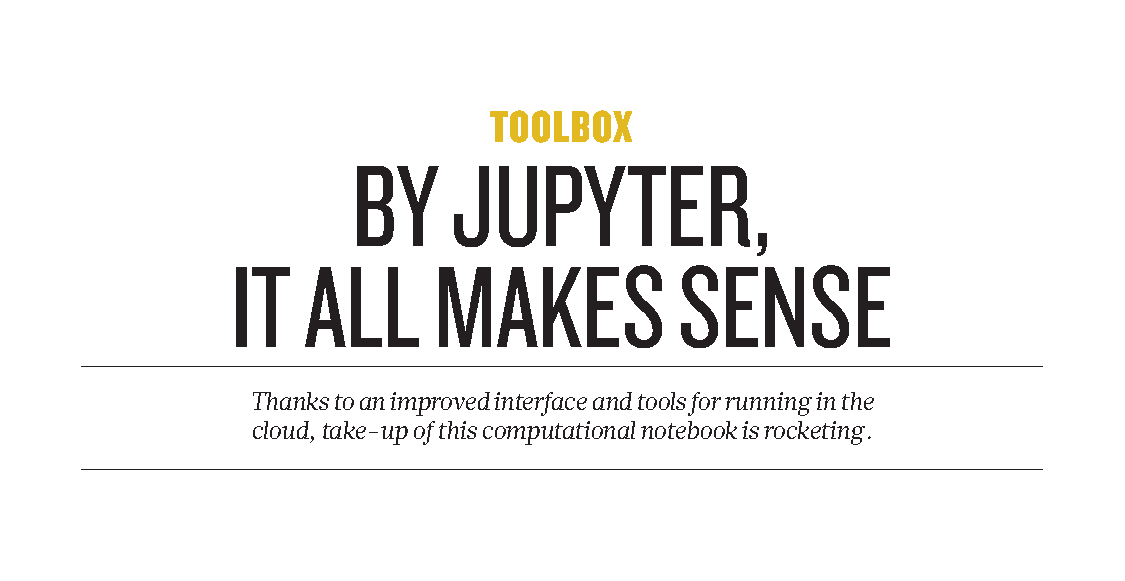
\includegraphics[width=\textwidth]{img/nature.pdf}
}
\only<2-3>{\it
      ``We went from Jupyter notebooks not existing some six years ago to in essence everybody~using~them~today''
}
\only<3>{\it
{
~\\
~\\
“I’ve never seen any migration [from...] this fast.\\ It’s just amazing”} 
}
\only<4>{\it
    ``notebooks have been around for decades, but...\\\  redesigned architecture that allows the notebook to speak dozens of programming languages ...  Julia (Ju), Python (Py) and R ...''
}
\only<5>{\it
\begin{columns}
\begin{column}{1.1\textwidth}\centering
    ``Researchers can also use notebooks to create tutorials or  interactive {\bf manuals for their software}\\ 
    ~[...]~
    ~\\ they can use notebooks to prepare  manuscripts, or~as~{\bf\emph teaching aids}''
\end{column}
\end{columns}
    }
% \only<5>{\it
%     ``[...] the ease with which notebooks facilitate access to remote data that might otherwise be impractical to download''
% }

   
\end{center}
}

\frame{
\begin{center}
\pgfimage[width=.8\textwidth]{img/pysdm_docs}\\
(\href{https://open-atmos.github.io/PySDM}{PySDM docs}, landing site visualisation by Ola Strząbała)
\end{center}
}

\frame{
  \frametitle{PySDM \& PyMPDATA examples with Colab}
  \href{https://open-atmos.github.io/PySDM/PySDM_examples/Pierchala_et_al_2022.html}{\pgfimage[width=\textwidth]{img/pierchala}}
}

\frame{
  \begin{center}
    \pgfimage[width=.9\textwidth]{img/examples_pypi}
  \end{center}
}

\frame{
  \frametitle{Perkel 2021, {\it Nature}  DOI: \href{https://doi.org/10.1038/d41586-021-01174-w}{10.1038/d41586-021-01174-w}\\ beyond single user \& caveats...}
  \pgfimage[width=\textwidth]{img/nature2021}
}
\frame{
  \frametitle{Perkel 2021, {\it Nature}  DOI: \href{https://doi.org/10.1038/d41586-021-01174-w}{10.1038/d41586-021-01174-w}\\ beyond single user \& caveats...} 
  \begin{center}
  \only<1>{\it\huge
      “If you do really great science but [...] no one gets access to it, then what’s the point?”
}
\end{center}
}


\frame{
\frametitle{Perkel 2021, {\it Nature}  DOI: \href{https://doi.org/10.1038/d41586-021-01174-w}{10.1038/d41586-021-01174-w}\\ beyond single user \& caveats...}
\begin{center}\it\huge
    ``Jupyter notebooks also encourage poor coding practice [...] difficult to organize code logically,\\
    ~\\
    break it into reusable modules and develop tests to ensure the code is working properly.''
\end{center}
}


\frame{
  \begin{center}
    \pgfimage[width=.9\textwidth]{img/oaju_pypi}
  \end{center}
}


\frame{
\begin{center}
    \bf import open\_atmos\_jupyter\_utils as oaju
\end{center}
\vspace{-1.5em}

    \begin{columns}[t]
        \begin{column}{.4\textwidth}
        \centering
            \begin{block}{\bf oaju.show\_plot()}
              \begin{itemize}
                  \item gives SVG inline graphics
                  \item adds save-SVG/PDF buttons
                  \item Google-Drive link on Colab
                  \item renders OK on GitHub
              \end{itemize}
              \begin{center}
              \pgfimage[height=.5\textheight]{img/sshot_colab}                 
              \end{center}
              \vspace{-1em}
            \end{block}
        \end{column}
        \begin{column}{.6\textwidth}{
            \begin{block}{\bf oaju.show\_anim() {\color{gray}(kudos Michał Wroński!)}}
              \begin{itemize}
                  \item uses matplotlib \& imageio
                  \item GIF$\leadsto$base64$\leadsto$.ipynb JSON
                  \item save-as-GIF button +Colab
                  \item renders OK on GitHub
              \end{itemize}
              \vspace{.05em}
              \begin{center}
              \pgfimage[height=.5\textheight]{img/sshot_anim}
              \end{center}
              \vspace{-1em}
            \end{block}
            }
        \end{column}
    \end{columns}
}


\frame{
\frametitle{Perkel 2021, {\it Nature}  DOI: \href{https://doi.org/10.1038/d41586-021-01174-w}{10.1038/d41586-021-01174-w}\\ beyond single user \& caveats...}
\begin{center}\it\huge
    ``And they are difficult to share, collaborate on and {\bf reproduce}''
\end{center}
}

\frame{
\frametitle{\bf oaju{\color{black}.}notebook\_vars{\color{black}()}{\footnote{\href{https://github.com/nteract/testbook}{\color{gray}similar to: pypi.org/p/testbook}}}}
\begin{columns}[t]
\begin{column}{0.5\textwidth}
    \begin{itemize}
        \item executes notebook code
        \item returns all locals as a dict
        \item option for plots on/off
        \item run-once/multiple asserts\\ ~~(using pytest fixture)
    \end{itemize}
\end{column}
\begin{column}{0.5\textwidth}
\vspace{-2em}
\begin{center}
    \pgfimage[width=\textwidth]{img/s_shot_test}
\end{center}
\vspace{-.5em} 
\end{column}

\end{columns}
}


\frame{
\frametitle{Perkel 2021, {\it Nature}  DOI: \href{https://doi.org/10.1038/d41586-021-01174-w}{10.1038/d41586-021-01174-w}\\ beyond single user \& caveats...}
\begin{center}\it\huge
        ``Many commercial platforms also address another notebook challenge: version control.''
\end{center}
}

\frame{
\pgfimage[width=\textwidth]{img/feature}

\href{https://github.com/open-atmos/PySDM/pull/1542/files}{$\leadsto$ sample PySDM Pull Request}

}


% \frame{
%   \frametitle{Jupyter notebooks in PySDM \& PyMPDATA}
%   \begin{itemize}
%       \item examples, tutorials
%       \item scenarios for tests
%       \item paper reproducers
%       \item closely integrated with project maintenance
%   \end{itemize}
% }





\frame{
  \begin{block}{take home messages:}
    \begin{itemize}
        \item<2-> ``{\it by Jupyter, it all makes sense!}\,'' 
        \item<3-> maintaining Jupyter notebooks with GitHub Actions: a rewarding challenge 
        \item<4-> try out \alert{open-atmos-jupyter-utils} yourself (feedback warmly welcome!)
        \item<5-> open-atmos projects welcome new contributors (also as Eng/MSc projects)
    \end{itemize}
  \end{block}

  \vspace{2em}

  \uncover<6->{
  \begin{center}
    \pgfimage[width=.75\textwidth]{img/logo-poziom-en-crop}
  \end{center}
  }

  \vspace{2em}

  \uncover<7->{
  \begin{center}
    Thank you for your attention!
  \end{center}
  }
}


\end{document}
